\documentclass[conference]{IEEEtran}

\usepackage[british]{babel}
\usepackage{cite}
\usepackage{graphicx}
\usepackage[hyphens]{url}
%\usepackage[pdftex]{hyperref}


% correct bad hyphenation here
%\hyphenation{op-tical net-works semi-conduc-tor}


\begin{document}
%
% paper title
% can use linebreaks \\ within to get better formatting as desired
\title{The Smart City from a Public Value Perspective}


% author names and affiliations
% use a multiple column layout for up to three different
% affiliations
\author{\IEEEauthorblockN{Ellie Cosgrave}
\IEEEauthorblockA{Department of Science, Technology,\\
Engineering \& Public Policy\\
UCL, UK\\
Email: e.cosgrave@ucl.ac.uk}
\and
\IEEEauthorblockN{Theo Tryfonas}
\IEEEauthorblockA{Faculty of Engineering\\
University of Bristol\\
Bristol, UK\\
Email: theo.tryfonas@bristol.ac.uk}
\and
\IEEEauthorblockN{Tom Crick}
\IEEEauthorblockA{Department of Computing\\
Cardiff Metropolitan University\\
Cardiff, UK\\
Email: tcrick@cardiffmet.ac.uk}}

% conference papers do not typically use \thanks and this command
% is locked out in conference mode. If really needed, such as for
% the acknowledgment of grants, issue a \IEEEoverridecommandlockouts
% after \documentclass


% use for special paper notices
%\IEEEspecialpapernotice{(Invited Paper)}


% make the title area
\maketitle


\begin{abstract}
This paper explores whether it is useful to view the fundamental ideas
behind the smart city concept through the lens of the `Public Value
Management' (PVM) paradigm. It investigates how appropriate ICT
investment in cities might be articulated and valued through the
concept of PVM. In order to achieve this, it explores the core
concepts found in the PVM literature, and draws key connections to the
smart city literature. This data is supported through semi-structured
interviews with smart city experts. The aim is to understand the
potential value of smart city concepts beyond simple optimisation of
city processes and cost cutting. This paper concludes that there are
conceptual connections between the PVM paradigm and the smart city. It
argues that the types of projects adopted, and their success, are
inseparable from the political paradigm within which they are
undertaken. As such, it takes the view that adopting the PVM paradigm
could support the successful delivery of smart cities, predominantly
through the ability to understand value beyond the optimisation of
systems.
% Index Terms fudge
\newline\newline
\indent {\textbf{Index Terms---Smart Cities, Public Value Management, Leadership, Information
Marketplaces, Sustainability}}
\end{abstract}

% For peer review papers, you can put extra information on the cover
% page as needed:
% \ifCLASSOPTIONpeerreview
% \begin{center} \bfseries Smart Cities, Public Value Management, Leadership, information marketplaces \end{center}
% \fi
%
% For peerreview papers, this IEEEtran command inserts a page break and
% creates the second title. It will be ignored for other modes.
%\IEEEpeerreviewmaketitle

% \begin{IEEEkeywords}
% Smart Cities, Public Value Management, Leadership, Information
% Marketplaces, Sustainability
% \end{IEEEkeywords}

\section{Introduction}

\subsection{Aims}
This paper explores whether it is useful to view the fundamental ideas
behind the smart city concept through the lens of the `Public Value
Management' (PVM) paradigm. It investigates how appropriate ICT
investment in cities might be articulated and valued through the
concept of PVM. In order to achieve this, it explores the core
concepts found in the PVM literature, and draws key connections to the
smart city literature. The aim is to understand the potential value of
smart city concepts beyond simple optimisation of city processes and
cost cutting.

This paper aims to draw tangible links between contemporary public
management concepts and ICT innovation. It is intended that this will
support city leaders in identifying areas of value from ICT investment
that cannot be uncovered by more traditional business case analysis.

\subsection{Methodology}
This paper uses the PVM paradigm as an interpretation instrument to
delineate useful links between the often quite abstract concepts
discussed in the smart city literature, and the realities of local
government delivery. This interpretivist research paradigm is
supported by an action research and grounded theory approach. A
literature review has been undertaken, which is supported by in-depth
semi-structured interviews with several leading smart city
experts. The purpose of this data collection was to focus on the core
themes in the smart city theory, the espoused value, and the
implications and challenges for city leadership in the interpretation
and delivery of this value.

This paper is part of a wider action research project that
investigates the steps that city leaders can take in order to maximise
the social, environmental and economic benefits of ICT in their
municipalities. This is achieved through working closely with city
leadership, as well as economists, technologists and service
providers. Increasingly, there is a strong theme of sustainability: the
role and impact of the transformational power of ICT for making our
world more sustainable.


\subsection{Context}
We live in a world transformed by technology, a trend started in the
industrial revolution that will extend long beyond our
lifetimes. However, over the last 10 years or so there has been a
significant shift in the nature of this development. Recent
advancements in information \& communications technology (ICT) have
seen the scale and role of data and information in every aspect of
modern life expand almost exponentially. This information is
transforming how we live our lives through better informed decision
making that is both conscious to us and invisible to us (via
automation/sensors e.g. in smart grids). This transformation has
driven increased speculation and research into the implications of ICT
on the way a city functions and operates~\cite{odensaal:2003} -- a
dialogue that has largely been captured in the smart city debate.

The transformation to `smart' is manifest not only in the operational
efficiency and optimisation heralded by ubiquitous sensors and
actuators, but it has also already altered global supply chains,
business models, and the way communities and individuals choose to
live their lives~\cite{komninos:2002}. Cities compete with each other
to attract private finance and investment within a national and global
`system of cities'. For example, the UK Government's Foresight project
The Future of
Cities~\footnote{\url{http://www.bis.gov.uk/foresight/our-work/projects/current-projects/future-of-cities}}
(launched in 2013), will take a long-term look at how UK cities can
best contribute to economic growth over the coming decade, taking into
consideration wellbeing, equity and social inclusion, all vitally
important for cities and their citizens. New ICT (such as smart
phones, broadband, 3G), has driven a fundamental change in the way we
work (networking through social media, distance working), how we shop
(online, price comparison), interact with family and friends (Skype,
social media), and our expectations of government (311, open
data). ICT has also been at the forefront of a new era of activism and
community unity. ``In the Arab Spring, social media facilitated action
in the Middle East and North Africa (MENA) region, providing a free
and accessible method of organising and coordinating
demonstrations''~\cite{bright:2011}. This was echoed in the 2011
London riots, and the subsequent clean-up operation.

Private sector technology companies like Facebook, Amazon and Google
have capitalised on this opportunity by using information to provide
value to their customers. These companies utilise information as a
core asset, and leverage it to create products and services that
respond to user desires and expectations. As highlighted in the report
``Information Marketplaces: The New Economics of Cities'' the current
`information marketplace' in cities already creates value for citizens
and contributes to its
sustainability~\cite{arup-et-al:2011}. Innovative information-based
products and services create jobs and support citizens in navigating
and using the city in effective, resource efficient and enjoyable
ways, as well as enabling sustainable
development~\cite{consustict:2008,ciscoconcities:2010}. In fact, the
`Smart 2020' report, written as part of The Climate Group's `Clean
Revolution' campaign, found that ICT-enabled interventions could
deliver ``7.8 GtCO$_2$e of emissions savings in 2020. This represents
15\% of emissions in 2020 based on BAU
estimation''~\cite{smart2020:2008}.

However, city leaders are struggling to identify the true sources of
value that novel ICT can generate for their municipalities. They are
finding it difficult to transform the higher-level concepts evident in
the smart city literature into actionable and effective policies,
projects and programs that deliver measureable value to the
citizenry~\cite{hollands:2008}. This is in part due to the nature of
the city itself, which is ``an enormously complex and open-ended
system, with many intertwining force fields influencing its form
simultaneously''~\cite{sevtsuk+beinart:2005}.

There is also a fundamental misunderstanding of the nature of the
change that is occurring. ICT can be used to increase the operational
efficiency of a city through applications such as traffic management
systems or the implementation of smart grid. However, more than that,
ICT is essential in creating a novel and dynamic marketplace that can
provide real long term value to the citizenry, both through the
services it provides and the continued economic development that it
facilitates. City leaders can use this concept to better understand
how to engage with ICT, and the smart city to enable them to deliver
real value to the modern public. This is a priority theme for the
Future Cities
Catapult~\footnote{\url{https://futurecities.catapult.org.uk}}, a
global centre of excellence on urban innovation, launched by the UK's
Technology Strategy Board in 2013.

Identifying the specific role of new ICT in such a complex system
requires a really fundamental understanding of the specific city
context, as well as a firm grasp of the vast array of roles for ICT in
delivering value to the city. Unfortunately, these two core
requirements are rarely found in the same place, and necessitate
effective cross-sector engagement, dialogue and action. Volker
Buscher, Director of Smart Cities at Arup explains:

\begin{quote}
{\emph{Effective, appropriate and insightful dialogue is required between
city leaders, smart city experts, and the wider community if the
complex problems faced by cities today are to be resolved. No single
party holds the full set of tools to make informed, appropriate and
innovative decisions that can address our contemporary local and
global issues...I see a great opportunity for cities to use smart city
ideas to transform themselves into thriving, healthy and happy places
that are globally competitive. But it will require sensitive and
informed dialogue that can be translated into action.}}~\cite{buscher:2012}
\end{quote}


\section{Public Value Management Paradigm}
The concept of Public Value Management (PVM) has grown out of and
developed upon the New Public Management (NPM) paradigm. ``Much of the
NPM literature is clear about the deficiencies yet NPM has remained
the dominant policy model in the public sector for over 20
years''~\cite{coleman:2011}.  NPM broadly asserts that market forces
can be leveraged to deliver more cost effective and efficient services
to citizens, and focuses on the utilisation of metrics and monitoring
to evaluate success.

Hefetz and Warner argue however, ``the social values inherent in
public services may not be adequately addressed by the economic
efficiency calculus of markets''~\cite{hefetz+warner:2004}. In
response to this, PVM takes a more pragmatic approach to the delivery
of public services and ``presents the achievement of public value as
its core objective''~\cite{stoker:2006}. It seeks to take into account
a wider variety of factors when deciding when and how to deliver
services, incorporating concepts beyond simple cost cutting. ``Public
Value has been described as a multi-dimensional construct -- a
reflection of collectively expressed, politically mediated preferences
consumed by the citizenry-created not just through `outcomes' but also
through processes which may generate trust or
fairness''~\cite{oflynn:2007}.

Horner and Hazel define Public Value as the correlate of private value
or shareholder return: ``The value may be calculated through economic
prosperity, social cohesion or cultural development. Ultimately, the
value -- such as better services, enhanced trust or social capital, or
social problems diminished or avoided -- is determined by the
citizen''~\cite{horner+hazel:2005}. This is a distinct step away from
the Net Present Value (NPV) approach, which attempts to gauge success
through the analysis of measures and metrics.

``Public Value Management does offer a new paradigm and a different
narrative of reform. Its strength lies in its redefinitions of how to
meet challenges of efficiency, accountability, and equity and in its
ability to point to a motivational force that does not rely on rules
or incentives to drive public service reform''~\cite{stoker:2006}.

``The `Public Value' approach has fast become an established (if as
yet minority) approach to assessing the success (or otherwise) of
public services and organisations in the UK, Australia and some other
countries''~\cite{talbot:2008}. It represents an approach that appears
to be feasible and realisable, and is therefore appropriate for a more
detailed investigation.

\subsection{Core Themes}
The PVM paradigm relies on the public sector gaining a legitimate
mandate for action, which is considered to be the only justification
for government action. Gaining this legitimacy requires a combination
of:

\begin{itemize} 
\item Performing efficiently;
\item Being accountable;
\item Being responsive to public needs;
\item And gaining trust.
\end{itemize}

Of course, these parameters are interrelated, but a focus on each of
these is required by the PVM paradigm if public sector actors are to
gain and maintain a mandate for action.

This legitimacy provides an opportunity for public managers to stretch
their traditional politically-driven mandate for action, and align
actions more closely with genuine public needs. ``The Public Value
approach suggests that actually public managers need not be so
passive -- that they can supplement and enhance the link between citizen
and delivery within the context of continued accountability to the
political principle and awareness of the wider authorising
environment''~\cite{gains+stoker:2009}.

\subsection{Performing Efficiently}
Although cost cutting is not the primary focus of PVM, the efficient
and appropriate use of resources is an imperative for ensuring
legitimacy in public sector actions. This means that city leaders must
seek to increase the efficiency of their operations and services, as
well as ensuring that new projects invested in represent the ‘best
value’ in the longer term. This includes the requirement to consider
the through-life implications of projects and programs including the
end-of-life transferability and adaptability of the scheme as
highlighted in cradle-to-cradle
thinking~\cite{mcdonough+braungart:2009}.

Furthermore, the PVM paradigm challenges leaders to think more deeply
about the services they choose to provide to their citizens. As Stoker
argues, simply ``providing services is no longer a sufficient
justification for state intervention funded by citizens, whether those
services are provided directly or
commissioned''~\cite{stoker:2006}. Instead, city leaders must evaluate
their role in delivering the value that those services traditionally
represented. For example, the city might have a responsibility to
ensure that their citizens are educated. In the past, this has been
interpreted as a mandate to run schools, and other education
services. The PVM paradigm calls for cities to consider how best to
deliver education in a city, rather than how best to run education
services. It focuses on value creation rather than service
delivery. This frees up city leaders to be more creative and
responsive to local needs.

Importantly this does not dictate a particular political path or
tendency. Baptista argues that the opportunities created by the smart
city ``may lead us to a more fundamental choice between a privatised
government (in which most issues are dealt with according to
commercial relationships and principles, with services paid for by
clients) and traditional, public government (in which many services
considered to be of public interest are provided to citizens and
businesses according to a variety of criteria not necessarily linked
to commercial considerations)''~\cite{baptista:2005}. However, ``city
leaders must take care to ensure that the ability of ICT to outsource
city services does not dictate the political direction, but that
instead, investment in ICT is derived from a sound articulation of
political, social and cultural values''~\cite{cosgrave+tryfonas:2012}.

The PVM paradigm calls for leadership to consider the role that they
should play in delivering public value in order to achieve policy
goals. While the PVM approach may lead to the adoption of a similar
project or program (i.e. a service-oriented approach to delivery), the
conceptual leap is important as it releases opportunities for the
creation of value beyond the traditional service approach. In this
way, ``the public value paradigm demands a commitment to goals that
are more stretching for public managers than those envisaged under
previous management regimes''~\cite{stoker:2006}. Furthermore, Kearns
argues that ``[Public Value] can be used both as an aid to judgment by
governments when deciding what activities to undertake as a yardstick
against which to access government
performance''~\cite{kearns:2004}. In this way, the PVM paradigm is
reflexive, and can be used to both define and gauge the success of
government investment.

\subsection{Being Accountable}
In order to achieve legitimacy, the public sector must show itself to
be transparent and accountable. ``Public value argues that public
services are distinctive because they are characterised by claims of
rights by citizens to services that have been authorised and funded
through some democratic process''~\cite{coats+passmore:2008}. This
democratically appointed authority means that public sector decision
makers are accountable to the public.

The political move towards accountability and openness has accelerated
in recent years. ``In his first day in office, President Barack Obama
issued the open government directive committing his government to the
three principles of transparency, participation and collaboration as
the cornerstone of an open data
government''~\cite{coleman:2011}. January 2010 saw the official launch
of data.gov.uk~\footnote{\url{http://data.gov.uk/}} (``{\emph{Opening up
Government}}''), releasing public data to help people understand how
government works and how policies are made. Similarly, the 2010 UK
Conservative Party manifesto claimed that the party intended to ``make
government more transparent''~\cite{conparty:2010}.

This move to transparency and accountability as the foundation for
public sector action has been partly in response to a general push for
a more open approach to governance, particularly around the topic of
open data. This has been compounded by increasing media scrutiny of
government in recent years, particularly through social media. In this
way, ``The same technological advances which have opened informatory
access and accountability of public services also can cause intense
pressure on public managers for managing demand and
expectations''~\cite{gains+stoker:2009}.  Moreover, ``because of
rising expectations, technological advances and 24-hour media scrutiny
the exchanges between politicians, managers and the public are of
greater intensity and any confusion in roles become politically
salient and can feed into a loss of public confidence about the
stewardship of both manager and
politician''~\cite{gains+stoker:2009}. To combat this, the public
sector has had to respond creatively to how it engages with and
incorporates public values into their decision-making processes.


\subsection{Being Responsive to Public Needs}
The PVM paradigm acknowledges that public leaders are operating in a
complex and evolving environment. In this light it argues that leaders
must adopt a dynamic approach to stakeholder engagement and
longer-term decision making, being responsive in the light of
complexity. This is not to say that governments should not plan ahead
and lay down concrete strategies, but that the strategies that they do
employ must take into account that the context that the strategy is
enacted in will change over time.  An understanding of this must be
incorporated into the strategy in order to make it more robust in the
longer term. ``The adoption of a public value approach to public
services needs to take account of both empirical complexities in the
delivery landscape and in how the rules of engagement between
politicians and managers are interpreted and
enacted''~\cite{gains+stoker:2009}.

Here, the relationship internally within local authorities is key, but
there is also a clear need for genuine dialogue with citizens. This
dialogue must be carried out in a way that reflects the diversity of
citizen needs, values and aspirations in an appropriate way. It must
also ensure that dialogue is set up in a way that enables it to be
incorporated into government planning and policy. This means that it
must be timely, specific and seek genuine insight.

\subsection{Gaining Trust}
All claims to legitimate action are founded on an underlying trust
between core actors. This is achieved through processes such as being
responsive, accountable, and efficient, but also requires effective
communication. A report from the Work Foundation on measuring Public
Value, puts trust and legitimacy at the center of their model. It
claims ``trust and legitimacy is placed at the top of this list
deliberately, in line with the Public Value approach, because without
it none of the other (aspects of public value) are
possible''~\cite{talbot:2008}. Likewise, in this paper, we argue
that the development of trust in government and governance decisions
is an imperative for successful public sector leadership.


\section{The Core Principles of Smart Cities}
The concept of the smart city has gained traction in recent years
and although it has been coined for a variety of purposes, it broadly
refers to a city that is using new ICTs innovatively and strategically
to achieve their aims. This should not necessarily be interpreted as
top-down vision delivered solely through government investment.  Quite
the opposite, the smart city is largely an organic `system of
systems'~\cite{harrison+abbottdonnelly:2011} which comprises an
ecosystem of products, services, companies, people and society that
are working together creatively to foster innovation within the
city. ``Smart cities cannot be defined by one application, or central
organising body, that sets pre-programmed limits. They will be defined
by individual citizens, who are anxious to collaborate with each
other...to create devices and applications that solve specific
problems. Smart cities will be places that foster creativity, where
citizens are generators of ideas, services and solutions, rather than
passive recipients of them''~\cite{haque:2012}.

A clear example of the evolution of this information marketplace is
the website Openly Local~\footnote{\url{http://openlylocal.com/}},
which scrapes data from various local government sources, and brings
it together in one accessible place, in order to create an ``open and
unified way of accessing Local Government information''. This
information can then be used for a variety of purposes, including the
development of innovative products and services for citizens.

While city leaders and local authorities are key stakeholders in this
system, they can by no means directly conduct and control this
marketplace. However, they have a responsibility to determine what
their role might be in fostering a healthy marketplace that can
support the delivery of their objectives. This involves investigating
how they should invest, at what time and for what purpose.

In that light, it is helpful for governments to adopt an understanding
of smart cities that lies beyond the optimisation of city
services. Working with the Smart Cities team at Arup over the past two
years, this research has explored the concept of the smart city
through a variety of meetings, workshops and practical
applications. Through this engagement, three core interrelated
categories of smart city value have
emerged~\cite{arup-et-al:2011,cosgrave-et-al:2013}. These are broadly:

\begin{itemize} 
\item Optimisation;
\item Service Innovation;
\item Information Marketplace.
\end{itemize}

Each category represents a different tier of conceptual integration of
themes and ideas. While `optimisation' looks quite specifically at the
operational efficiency of a given system, the development of an
`information marketplace' integrates many system externalities, and
deals with a wider variety of themes.

\subsection{Optimisation}
Many people and organisations have pushed the idea that the smart
city, revolved around ubiquitous sensing and actuation, can deliver
optimisation of city services. For example, a Forrester report
describes the smart city as ``A city that uses information and
communications technologies to make the critical infrastructure
components and services of a city…more aware, interactive, and
efficient''~\cite{belissent:2010}. There is a significant focus on the
use of ICT improve the operational efficiency, or in reducing
provisioning costs of core city services. This is exemplified by smart
grid projects. Here, information is collected in real time about the
energy usage at different areas of the grid. This information is then
used to optimise the flows in the system. Some smart grids have
actuation functionality that enables them to balance the load on the
grid -- thereby reducing peak requirements.

The word `optimisation' has been tangled up in significant debate when
referring to engineered systems; the move towards a `fully optimised'
approach to systems has led to the increased vulnerability of systems
by the tendency to engineer-out redundancy. This can lead to single
point of failure systems that are not resilient to change, and cannot
cope with unexpected events.

In this paper, we to refer to optimisation in the sense of making
improvements to a system in such a way that is most suited to the
delivery of its purpose. This does require a focus on resource
efficiency, but also incorporates process improvement, and building up
resilience to unexpected events through access to more granular
information about the real-time state of the system. In this way,
optimisation should be understood in terms of improving the quality of
the services provided, at lower resource cost, and with increased
resilience to failure.

City service optimisation is an internally focused area for cities,
where they investigate ways in which their internal processes and
functioning can be achieved more effectively. Chris Namih, Consultant
(Smart Cities) at Arup, explains that:

\begin{quote}
{\emph{Optimisation is internal within the provision of services as they
stand.}}~\cite{namih:2012}
\end{quote}

\subsection{Service Innovation}
The concept of service innovation in smart cities includes the
development of novel ways of delivering service outcomes in the
city. This goes beyond optimisation, offering a paradigm shift in the
way that services are delivered, rather than improving (or
`optimising') within a given way of doing things. It offers new and
more innovative ways of delivering services within the city.

A service innovation will have an implication for the way in which a
user behaves, or experiences the city. An example of this might be the
move to a smart ticketing system for public transport within the
city. Transport for London's Oyster card
system~\footnote{\url{http://www.tfl.gov.uk/tickets/14836.aspx}}
resulted in a transformation in the way people interacted with public
transport in several ways. Chiefly, flexible charging allowed people
to roam more freely around the city, particularly in going beyond the
zone for which they had bought a travel card. It also increased
efficiency of bus systems by significantly speeding up the boarding
time required.

The Oyster card data has also provided significant insight into user
behaviour~\cite{reades:2011}, which has been useful for research, and
system optimisation. The opportunities for this detailed dataset have
not yet been fully realised, but it is recognised that, if used
innovatively, it can be used to both optimise the system and
contribute to the information marketplace as described below.

\subsection{Information Marketplace}
The concept of the information marketplace argues that there is a
wider economy developing around the smart city that is outside the
boundaries of the local council. This marketplace relies on
information as a core asset to drive economic development and other
social and environmental aims. So, in the case of transport,
innovative companies or individuals could use anonymised oyster card
data to create novel products and services. The Information
marketplaces report argues, ``By unlocking technology, infrastructure
and public data, cities can open up new value chains that spawn
innovative applications and information products that make possible
sustainable modes of city living and
working''~\cite{arup-et-al:2011}. This concept is at the centre of
fostering the information marketplace. Chris Namih explains:

\begin{quote}
{\emph{For me an information marketplace... creates an ecosystem where third
parties can deliver services or certain aspects of them, or entirely
new services by being enabled by information.}}~\cite{namih:2012}
\end{quote}

Thus, fostering this ecosystem of benefits supports a city
in becoming more competitive, as well as achieving their core high
level objectives.

%\subsection{Conclusion}

\begin{quote}
{\emph{These buckets aren’t just technology-focused. You can optimise
through process change or business organisation change, and you can do
the same in service innovation. Technology is often involved, and
technology can lead to these changes, but it is not the only factor.}}~\cite{namih:2012}
\end{quote}

This means that the smart city concept is concerned with more than
just the implementation of technology. It is also concerned with the
ecosystem that can be built up around that technology in order to
create positive social, economic, environmental and political
outcomes. This requires both top-down engagement through hard
infrastructure investment and visioning, as well as a bottom-up energy
to capitalise upon and drive innovation in ICT and service provision.
 
The multiple layers of the smart city story means that, while
governments do have a significant role to play in the creation of
smart cities (particularly through the optimisation of city services)
there are a vast number of stakeholders that lie outside the bounds of
local government. This is particularly relevant to the creation of
information marketplaces within the city. As such, city leaders need
to understand how to engage with this evolving information community,
and understand their needs in relation to economic and social drivers,
as well as investing in the existing marketplace within their city.


\section{The public value lens: the relationship to smart cities}
Achieving city objectives through smart city projects requires
political and civil engagement. L\'{e}an Doody, Smart Cities Associate at
Arup, explains that effective action requires:

\begin{quote}
{\emph{A certain leadership in the council to look at the role of IT
information in achieving top level goals.}}~\cite{doody:2012}
\end{quote}

This does not exclude the importance of the bottom-up creation of
smart cities, but demonstrates that the types of projects that a city
engages/invests in, and their effectiveness, are inextricably linked
to the prevailing political and cultural paradigm.

Two-thirds of UK government ICT projects fail~\cite{postitp:2003},
partly due to the fact that ``city administrators often fail to
acknowledge projects as being complex or strategic and neglect many
`softer' issues that are essential for a project to
succeed''~\cite{arup-et-al:2011}. This high failure rate has also been
due to ICT providers under bidding in a competitive tendering process
in order to win work, leading to under-resourced and under-supported
projects. Measures have been put in place, for example the creation of
the Major Projects
Authority~\footnote{\url{https://www.gov.uk/government/groups/major-projects-authority}},
to improve project performance for the taxpayer, as well as the
creation of the Government Digital
Service~\footnote{\url{https://gds.blog.gov.uk/about/}} in 2010 to
implement the UK Government Digital
Strategy~\cite{ukgds:2013}. However, projects have failed as a result
of being largely driven by the creation of `political capital' for the
presiding politician, which may not have a rigorous founding in the
realities of successful project delivery.

ICT projects in cities cannot be seen as distinct from their
political, social, or economic context, and therefore must be analyzed
as part of that system. This section seeks to identify how the
political paradigm adopted in a city relates to the success of a smart
cities program, with a particular focus on PVM.

Figure~\ref{fig:smartcitypvm} maps the core themes discussed in the
PVM literature to the three `buckets' derived in the smart cities
section. Conceptualising the problem in this way highlights a two-way
relationship between PVM and smart cities. In one sense, new ICTs are
pushing the need for governments to adopt a PVM approach because of
increased media scrutiny and increased skepticism from the public. In
another sense, adopting a PVM approach could help city leaders to
understand the potential value of smart cities more comprehensively
and holistically.

\begin{figure}[!ht]
\centering
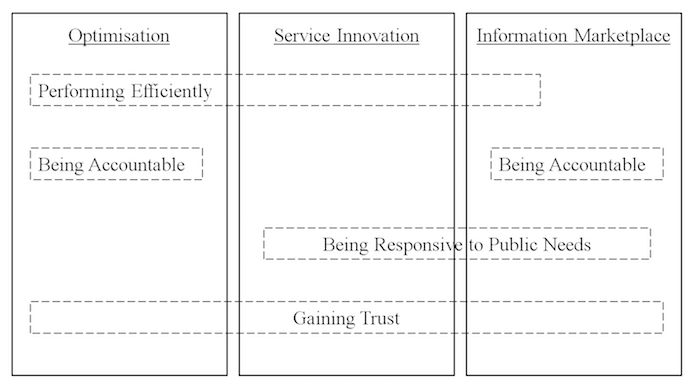
\includegraphics[width=\columnwidth]{smartcitypvm.png}
\caption{Relationship between the smart city and the public value management paradigm}
\label{fig:smartcitypvm} 
\end{figure}


\subsection{Performing Efficiently}
As previously discussed, the PVM paradigm espouses that efficient and
appropriate use of resources is a central tenet in public sector
legitimacy. There are multiple examples that highlight smart cities
contributing to resource efficiency in city service delivery (e.g. the
\'{A}guas de Cascais roll-out of `TaKaDu' which is a ``web-based service
that allows the water utility to detect leakage and network problems
as they occur''~\cite{prwebport:2012}).

The obvious link here is in the `optimisation' category of smart city
projects. These optimise city systems in order to reduce resource
consumption and deliver better services. However, because the PVM
paradigm calls governments to reassess how they provide value in the
city, a distinct crossover with the information marketplace
emerges. In the creation of the information marketplace, city leaders
need to understand how to foster public value in the wider city
ecosystem. This might be through investment in the technology sector,
fostering innovation through funded competitions (e.g. the Apps for
Democracy~\footnote{\url{http://www.appsfordemocracy.org/}}
competition in Washington, which ``yielded 47 web, iPhone and Facebook
apps in 30 days -- a \$2,300,000 value to the city at a cost of
\$50,000'', which was given to the developer of the winning app as a
prize) or running appropriate events and symposiums. This represents a
clear progression from the direct approach of delivering value
exclusively through public sector service provision, to an
understanding that value can also be derived through fostering
positive externalities.

As Chris Namih explains:

\begin{quote}
{\emph{In understanding the information marketplace, quite often it is the
mind-set that needs to be re-jigged.}}~\cite{namih:2012}
\end{quote}

The PVM approach supports this shift in focus by arguing for a more
holistic approach to value creation in the city that does not focus
solely on the delivery of services. In this way, an adoption of the
PVM approach may support leaders in capitalising on the information
marketplace.

\subsection{Being Accountable}
The PVM paradigm argues that in order to gain legitimacy, public
leaders must be accountable to the public. In reality however, while
governments and political leaders are often held accountable for
certain services, they have in some cases, given over the
responsibility for delivery over to third parties. This has restricted
their ability to impact upon, or change the way in which those
services are delivered. If governments are to have more control over
the public services that they are accountable for, they must think
creatively about how to engage with responsible parties. ICT may have
a role to play here in fostering better communications, or joining-up
infrastructure projects so that there is greater interrelationship.

The concept of accountability also assumes that there is an object or
body to whom a party is accountable. In the case of cities, this body
is the citizenry. If genuine accountability is to be demonstrated then
city leaders need to foster effective communication with citizens, in
a way that enables citizens to challenge and appreciate the ways in
which city leaders are accountable for their actions. As such,
accountability for public spending may require a more open approach to
governance. This may be in the form of opening up city dataset to the
public, which would in turn contribute to the information
marketplace. This demonstration of accountability is also heavily
linked to the fostering of trust as discussed in Section~\ref{sec:gaintrust}.

\subsection{Being Responsive to Public Needs}
A key part of the PVM paradigm is a responsive and reflexive approach
to the needs of the citizenry. Effective public dialogue that can be
fed into investment decisions is essential in achieving this. L\'{e}an
Doody, explains that one of the key principles of smart cities is:

\begin{quote}
{\emph{About making sure the flow of information is not just one way,
    so it’s about getting informed commentary and ideas back from the
    public...Technology platforms potentially have a huge role in
    enabling people to communicate directly. This opens up government
    at different levels, so it's a kind of flattening of the
    organisation and they way that people are able to communicate
    directly with maybe more junior people who actually have a voice
    now through Twitter or seem to be a bit more happy to engage.}}~\cite{doody:2012}
\end{quote}

Importantly, this interaction and understanding of citizen needs must
be translated into appropriate action and investment. In Los Angeles,
transport planners are using web platforms strategically in order to
engage with the public to inform their planning process. Part of this
includes a `virtual town hall' where subjects are opened up for
discussion over several days; this is accompanied by face-to-face
workshops. The diversity of consultation approaches means that the
city is able to capture a wider variety of citizens needs than would
have been previously possible. Importantly, the planners have a
structured plan to feed back findings to inform planning decisions at
the appropriate time in the process~\cite{la2b:2011}.


\subsection{Gaining Trust}\label{sec:gaintrust}
New ICT is also driving city leaders to a more open and transparent
approach. Increased media coverage has become so ubiquitous through
the rise of Web 2.0 and social media that governments are under
unprecedented levels of scrutiny. This has driven the political
transparency agenda, firstly in the US, and now increasingly in Europe
and elsewhere. Furthermore, now that the technology is at a level
where it really can be used to aggregate huge levels of personal data
about citizens and their behaviour, cities that do not take an open
approach may be accused of operating `big brother' type states. L\'{e}an
Doody explains that ubiquitous ICT and smart technologies:

\begin{quote}
{\emph{Would also allow a horrible dystopian view of the future- look
    at how technology is being used in more repressive regimes.}}~\cite{doody:2012}
\end{quote}

Citizens and organisations will start to question leaders that chose
to cut themselves and their operations off from public dialogue,
especially now that there are widespread technology platforms that
make engagement so much easier. The PVM paradigm's emphasis on being
accountable to citizens and gaining trust, is clearly going to play an
important part in managing the relationship between citizens and
public and political leaders, whether or not they have a desire to
engage with the transparency and open data movement.

Citizens can become quite sensitised to perceived privacy violations
with respect to their personal data. This has been exemplified by
Google's change in privacy policy which enabled them to
``cross-pollinate personal user data recorded on any of its 60
products''~\cite{pinterkrainer:2012}. This incited a severe reaction from the international
community: ``Lawmakers, privacy authorities, technical experts, and
privacy organizations around the world (released) public statements
and direct letters to Google representatives that (were) critical of
the new policy. Advocacy groups criticise(d) and condemn(ed) the
changes, and the European Union, Japanese, and Canadian privacy
authorities have released statements indicating that the new policy
may violate their domestic privacy laws''~\cite{sutton:2012}.

There are important lessons for any organisation that is in control of
significant amounts of public data, especially in public organisations
that are directly accountable to the public. Holders and users of
public data open up channels for the development of mistrust between
themselves and the public, which can severely damage long term
relationships, and consequently the effectiveness of public service
provision.

In order to combat this, city leaders must demonstrate trustworthiness
by becoming custodians of public data, utilising it only when they can
demonstrate a tangible link to the delivery of public value. This is a
complex task that requires further investigation.


\section{Conclusion} 
This paper has highlighted that there are conceptual connections
between the PVM paradigm and the concept of the smart city. It argues
that the types of projects adopted, and their success, are inseparable
from the political paradigm within which they are undertaken. As such,
it takes the view that adopting the PVM paradigm could support the
successful delivery of smart cities, predominantly through the ability
to understand value beyond optimization of systems.

The PVM paradigm encourages governments to conceptualise their actions
from a new perspective, requiring them to place the creation of public
value at the center of their focus, rather than the provision of
efficient services. This subtle shift in focus actually requires a
profound leap in the way in which decisions are made, and that value
from projects can be analysed. The PVM approach offers a key for city
leaders to understand the value of smart city projects, and
importantly provides a political legitimacy for investment in it. This
is especially important when city leaders are trying to justify
investment in the information marketplace. Here, certain values need
to be incorporated that are not measureable in the traditional sense
-- that do not sit neatly alongside traditional metrics, but that
require investment nonetheless.

If government is able to understand itself as a body that is dealing
with complexity, trying to be responsive to needs and think in the
long term, and not necessarily metric oriented, it can get more out of
smart cities. This is because it is able to articulate value that lies
beyond optimization and bottom line efficiencies. So, if city leaders
are able to look at ICT through a public value lens, it helps them to
understand the value of ICT projects and smart cities. From this
viewpoint city leaders can come to make better decisions, based on a
more coherent understanding of the role of technology in achieving
their core aims.

This paper identifies a two-way relationship between PVM and smart
city delivery. Firstly, new ICT (or smart city concepts) pushes the
need for governments to adopt the PVM paradigm through:

\begin{itemize}
\item Requirement for transparency;
\item Increased scrutiny from social media.
\end{itemize}

Equally, smart city concepts also support the delivery of public value through:

\begin{itemize}
\item Data provision (and open data);
\item Effective communication;
\item Supporting dynamic governance and ability to respond to citizen needs;
\item Dealing with complexity;
\item Fostering creativity.
\end{itemize}

The new perspective offered by PVM enables local government to
understand the value of smart city beyond efficiency gains that can be
achieved through optimisation. This paper argues that applying the
traditional NPM approach to smart cities restricts a city’s ability to
invest in ways that deliver the greatest value to the citizenry. This
is especially relevant for value that cannot always be measured
through standardized metrics and measures, or through bottom-line cost
cutting. For adequate smart city investment, city leaders must be able
to grapple with the real-life complexity of their challenge. They must
understand that the problems they face are multifaceted, interrelated
and dynamic. This necessitates the genuine public engagement,
effective internal communication and collaboration, and responsiveness
as represented in the PVM approach.

This paper argues that taking a public value management approach can
support cities in understanding the value of ICT investment, as well
as increasing the likelihood of success of smart city
interventions. However, it does not claim that adopting the PVM
paradigm is a requirement for smart city delivery, or that is holds
exclusivity over smart city implementation. There may well be other
management paradigms that support the delivery of smart city
concepts. As L\'{e}an Doody explains:

\begin{quote}
{\emph{I think the point about technology is that it is about your
intentions more than the technology, the technology will allow lots of
different outcomes.}}~\cite{doody:2012}
\end{quote}

Equally, we do not intended to claim that the adoption of PVM will
necessarily deliver valuable smart city interventions. This paper
merely means to highlight the potential value in viewing the delivery
of smart cities through a public value lens.

\section{Future work}
This paper is part of a wider action research project that
investigates the steps that city leaders can take in order to maximise
the social, environmental and economic benefits of ICT in their
municipalities. From a sustainable development perspective, we note
the imperative to connect {\emph{within}} cities (which, by inference,
includes technology) and the increasing importance of connecting
{\emph{among}} cities: a global community of connected cities
committed to sustainability. We intend to use the concepts developed
in this paper, and other work to continue to deepen our understanding
of the challenges faced by city leaders in approaching smart city
delivery.

Firstly, we intend to use this conceptual foundation to work with a
city to understand the implications of smart cities for their
investment and organisational decisions. We will take an action
research approach to develop a systems-based process/framework that
allows cities to find the cross sector implications of the smart city,
and guide decision-making.  Through interviews, case studies and
workshops, we will seek to identify the implications of the findings
for city leadership in terms of management processes and
organisational structure. Given the new understanding of the role of
technology, how might they now evaluate technology investment projects
in the future? Does it have an implication for the metrics they are
able to employ? What limitations and drawbacks might they still face?

\section*{Acknowledgment}
Part of this work has been supported by Arup and the University of
Bristol's Industrial Doctorate Centre in Systems (EPSRC Grant
EP/G037353/1). The first two authors would also like to thank Volker
Buscher and Professor John Davis for their support in preparing earlier
versions of this paper.

%\newpage

% trigger a \newpage just before the given reference
% number - used to balance the columns on the last page
% adjust value as needed - may need to be readjusted if
% the document is modified later
\IEEEtriggeratref{28}
% The "triggered" command can be changed if desired:
%\IEEEtriggercmd{\enlargethispage{-5in}}

% references section
\bibliographystyle{IEEEtran}
%\bibliography{ict4s2014}
\begin{thebibliography}{99}

\bibitem{odensaal:2003}
N.~Odendaal, ``Information and communication technology and local governance:
  understanding the difference between cities in developed and emerging
  economies,'' \emph{{Computers, Environment and Urban Systems}}, vol.~27,
  no.~6, pp. 585--607, 2003.

\bibitem{komninos:2002}
N.~Komninos, \emph{{Intelligent Cities: Innovation, Knowledge Systems and
  Digital Spaces}}.\hskip 1em plus 0.5em minus 0.4em\relax Routledge, 2002.

\bibitem{bright:2011}
P.~Bright, ``How the london riots showed us two sides of social networking,''
  August 2011,
  \url{http://arstechnica.com/tech-policy/news/2011/08/the-two-sides-of-social-networking-on-display-in-the-london-riots.ars}
  (accessed 2014-02-12).

\bibitem{arup-et-al:2011}
{Arup, The Climate Group, Accenture and Horizon, University of Nottingham},
  ``{Information Marketplaces: The New Economics of Cities},'',
  November 2011.

\bibitem{consustict:2008}
W.~Wagener, ``{Connected and Sustainable ICT Infrastructure},'' {Connected
  Urban Development}, 2008.

\bibitem{ciscoconcities:2010}
N.~Villa and S.~Mitchell, ``{Connecting Cities: Achieving Sustainability
  Through Innovation},'' {Cisco}, October 2010.

\bibitem{smart2020:2008}
{The Climate Group}, ``{SMART 2020: Enabling the low carbon economy in the
  information age},'' 2008, {Global eSustainability Initiative (GeSI)}.

\bibitem{hollands:2008}
R.~G. Hollands, ``Will the real smart city please stand up? intelligent,
  progressive or entrepreneurial?'' \emph{City}, vol.~12, no.~3, pp. 303--320,
  2008.

\bibitem{sevtsuk+beinart:2005}
A.~Sevtsuk and J.~Beinart, ``{The effects of ICT on City Form},'' {MIT School
  of Architecture and Planning}, 2005.

\bibitem{buscher:2012}
V.~Buscher, April 2012, {Interview}.

\bibitem{coleman:2011}
E.~Coleman, ``{From New Public Management to Open Governance: A New Future or
  The More Things Change the More They Stay The Same?}'' Master's thesis,
  University of Warwick, UK, 2011.

\bibitem{hefetz+warner:2004}
A.~Hefetz and M.~Warner, ``{Privatization and Its Reverse: Explaining the
  Dynamics of the Government Contracting Process},'' \emph{{Journal of Public
  Administration Research and Theory}}, vol.~14, no.~2, pp. 171--190, 2004.

\bibitem{stoker:2006}
G.~Stoker, ``{Public Value Management: A New Narrative for Networked
  Governance?}'' \emph{{The American Review of Public Administration}},
  vol.~36, no.~1, pp. 41--57, 2006.

\bibitem{oflynn:2007}
J.~O'Flynn, ``{From New Public Management to Public Value: Paradigmatic Change
  and Managerial Implications},'' \emph{{Australian Journal of Public
  Administration}}, vol.~66, no.~3, pp. 353--366, 2007.

\bibitem{horner+hazel:2005}
L.~Horner and L.~Hazel, ``{Adding Public Value},'' {The Work Foundation}, January 2005.

\bibitem{talbot:2008}
C.~Talbot, ``{Measuring Public Value -- A competing values approach},'' {The
  Work Foundation}, October 2008.

\bibitem{gains+stoker:2009}
F.~Gains and G.~Stoker, ``{Delivering `Public Value': Implications for
  Accountability and Legitimacy},'' \emph{{Parliamentary Affairs}}, vol.~62,
  no.~3, pp. 438--455, 2009.

\bibitem{mcdonough+braungart:2009}
W.~McDonough and M.~Braungart, \emph{{Cradle to Cradle: Remaking the Way We
  Make Things}}.\hskip 1em plus 0.5em minus 0.4em\relax {North Point Press},
  2002.

\bibitem{baptista:2005}
M.~Baptista, ``{e‑Government and State Reform: Policy Dilemmas for Europe},''
  \emph{{Electronic Journal of e-Government}}, vol.~3, no.~4, pp. 167--174,
  2005.

\bibitem{cosgrave+tryfonas:2012}
E.~Cosgrave and T.~Tryfonas, ``{Exploring the Relationship Between Smart City
  Policy and Implementation},'' in \emph{{Proceedings of the 1st International
  Conference on Smart Systems, Devices and Technologies (SMART 2012)}}, 2012,
  pp. 79--82.

\bibitem{kearns:2004}
I.~Kearns, ``{Public Value and E-Government},'' {Institute for Public Policy
  Research}, 2004.

\bibitem{coats+passmore:2008}
D.~Coats and E.~Passmore, ``{Public Value: The Next Steps in Public Service
  Reform},'' {The Work Foundation}, October 2008.

\bibitem{conparty:2010}
{The Conservative Party Manifesto}, ``{Why we think you should vote for us},'', 2010.

\bibitem{harrison+abbottdonnelly:2011}
C.~Harrison and I.~{Abbott Donnelly}, ``{A Theory of Smart Cities},'' in
  \emph{{Proceedings of the 55th Annual Meeting of the International Society
  for the Systems Sciences (ISSS)}}, 2011, pp. 7--22.

\bibitem{haque:2012}
U.~Haque, ``Surely there's a smarter approach to smart cities?'' April 2012,
  \url{http://www.wired.co.uk/news/archive/2012-04/17/potential-of-smarter-cities-beyond-ibm-and-cisco}
  (accessed 2014-02-12).

\bibitem{cosgrave-et-al:2013}
E.~Cosgrave, K.~Arbuthnot, and T.~Tryfonas, ``{Living Labs, Innovation
  Districts and Information Marketplaces: A Systems Approach for Smart
  Cities},'' in \emph{Proceedings of the 2013 Conference on Systems Engineering
  Research}, 2013, pp. 668--677.

\bibitem{belissent:2010}
J.~B\'{e}lissent, ``{Getting Clever About Smart Cities: New Opportunities
  Require New Business Models},'' {Forrester}, 2010.

\bibitem{namih:2012}
C.~Namih, April 2012, {Interview}.

\bibitem{reades:2011}
J.~Reades, ``{Early Views of Public Transit Usage in London},'' April 2011,
  \url{http://simulacra.blogs.casa.ucl.ac.uk/2011/04/early-views-of-public-transit-usage-in-london/}
  (accessed 2014-02-12).

\bibitem{doody:2012}
L.~Doody, April 2012, {Interview}.

\bibitem{postitp:2003}
{Parliamentary Office of Science and Technology}, ``{Government IT
  projects},'', Report 200, July 2003.

\bibitem{ukgds:2013}
{UK Government}, ``{Government Digital Strategy}'', December 2013, \url{https://www.gov.uk/government/publications/government-digital-strategy}
  (accessed 2014-02-12).

\bibitem{prwebport:2012}
{PRWeb}, ``{\'{A}guas de Cascais Rolls Out TaKaDu for Water Network Monitoring
  and Water Loss Reduction},'' March 2012,
  \url{http://www.prweb.com/releases/2012/3/prweb9288938.htm} (accessed
  2014-02-12).

\bibitem{la2b:2011}
{Los Angeles Departments of City Planning and Transportation}, ``{LA2B},''
  2011, \url{http://la2b.org/about/} (accessed 2014-02-12).

\bibitem{pinterkrainer:2012}
M.~Pinter-Krainer, ``{Google Enforces New Privacy Policy, Despite International
  Outcry About Its Implications},'' March 2012,
  \url{http://www.consumerwatchdog.org/story/google-enforces-new-privacy-policy-despite-international-outcry-about-its-implications}
  (accessed 2014-02-12).

\bibitem{sutton:2012}
M.~Sutton, ``{International Reactions to Google’s New Privacy Policy},''
  March 2012,
  \url{https://www.eff.org/deeplinks/2012/03/international-reactions-googles-new-privacy-policy}
  (accessed 2014-02-12).

\end{thebibliography}



% that's all folks
\end{document}


